\documentclass[a4paper, 12pt]{article}
\usepackage{amsmath}
\usepackage[tmargin=1.0in]{geometry}
\usepackage{enumitem}
\usepackage{algorithmic}
\usepackage{algorithm}
\usepackage{graphicx}
\usepackage{url}

\usepackage[colorlinks]{hyperref}
%\usepackage[colorlinks,citecolor=DeepPink4,linkcolor=DarkRed]{hyperref}
\usepackage{breakurl}
\usepackage{soul}
% *** Verbatim Environment ***
\usepackage{fancyvrb, color}


\definecolor{airforceblue}{rgb}{0.36, 0.54, 0.66}
\definecolor{paynesgrey}{rgb}{0.25, 0.25, 0.28}
\definecolor{royalblue}{rgb}{0.0, 0.14, 0.4}
\hypersetup{
  colorlinks   = true, %Colours links instead of ugly boxes
  urlcolor     = royalblue, %Colour for external hyperlinks
  linkcolor    = paynesgrey, %Colour of internal links
  citecolor   = red %Colour of citations
}
%%************************************************ Setup *****************************************/
%% Set the vertical layout of float pages
\makeatletter	
\setlength{\@fptop}{0pt}	% Distance from top of page to first float
\setlength\@fpsep{15pt}		% Separation between floats
\makeatother

%%********************************************* Metadata *****************************************/
\title{\vskip -3ex SSLProject: SSL/TLS Connection Indicator and Certificate Checker}
\author{\textit{Shuang Liang}}
\date{December 18, 2014}

%%****************************************** Document Entry **************************************/
\setlength\parindent{0pt}
\begin{document}
%%-----------------------------------------------------------------------------
%% 	Title
%%-----------------------------------------------------------------------------
%{\centering
%	{\Large SSLProject: SSL/TLS Connection Indicator and Certificate Checker}\\
%	{\hfill \textit{Shuang Liang \quad Dec. 18, 2014}}\\
%}
%\noindent
%\vskip 3ex
\maketitle
\tableofcontents
\clearpage

%%=============================================================================
%% 	SSL/TLS indicator
%%=============================================================================
\section{Android Apps secure connection indicator}
%%-----------------------------------------------------------------------------
%% 	Description
%%-----------------------------------------------------------------------------
\subsection{Project description}
Android Web applications use the padlock symbol ahead of the URL to indicate the current connection to the server
 is secure or not. But there's no padlock symbol for mobile apps on Android system. So we want to build the padlock 
 scheme on Android system to notify users the current app is communicating via a secured or unsecured connection.
 Figure \ref{fig:padlock} illustrates the padlock symbol to indicate secured or unsecured connection.
\begin{figure}[!htb]
\centering
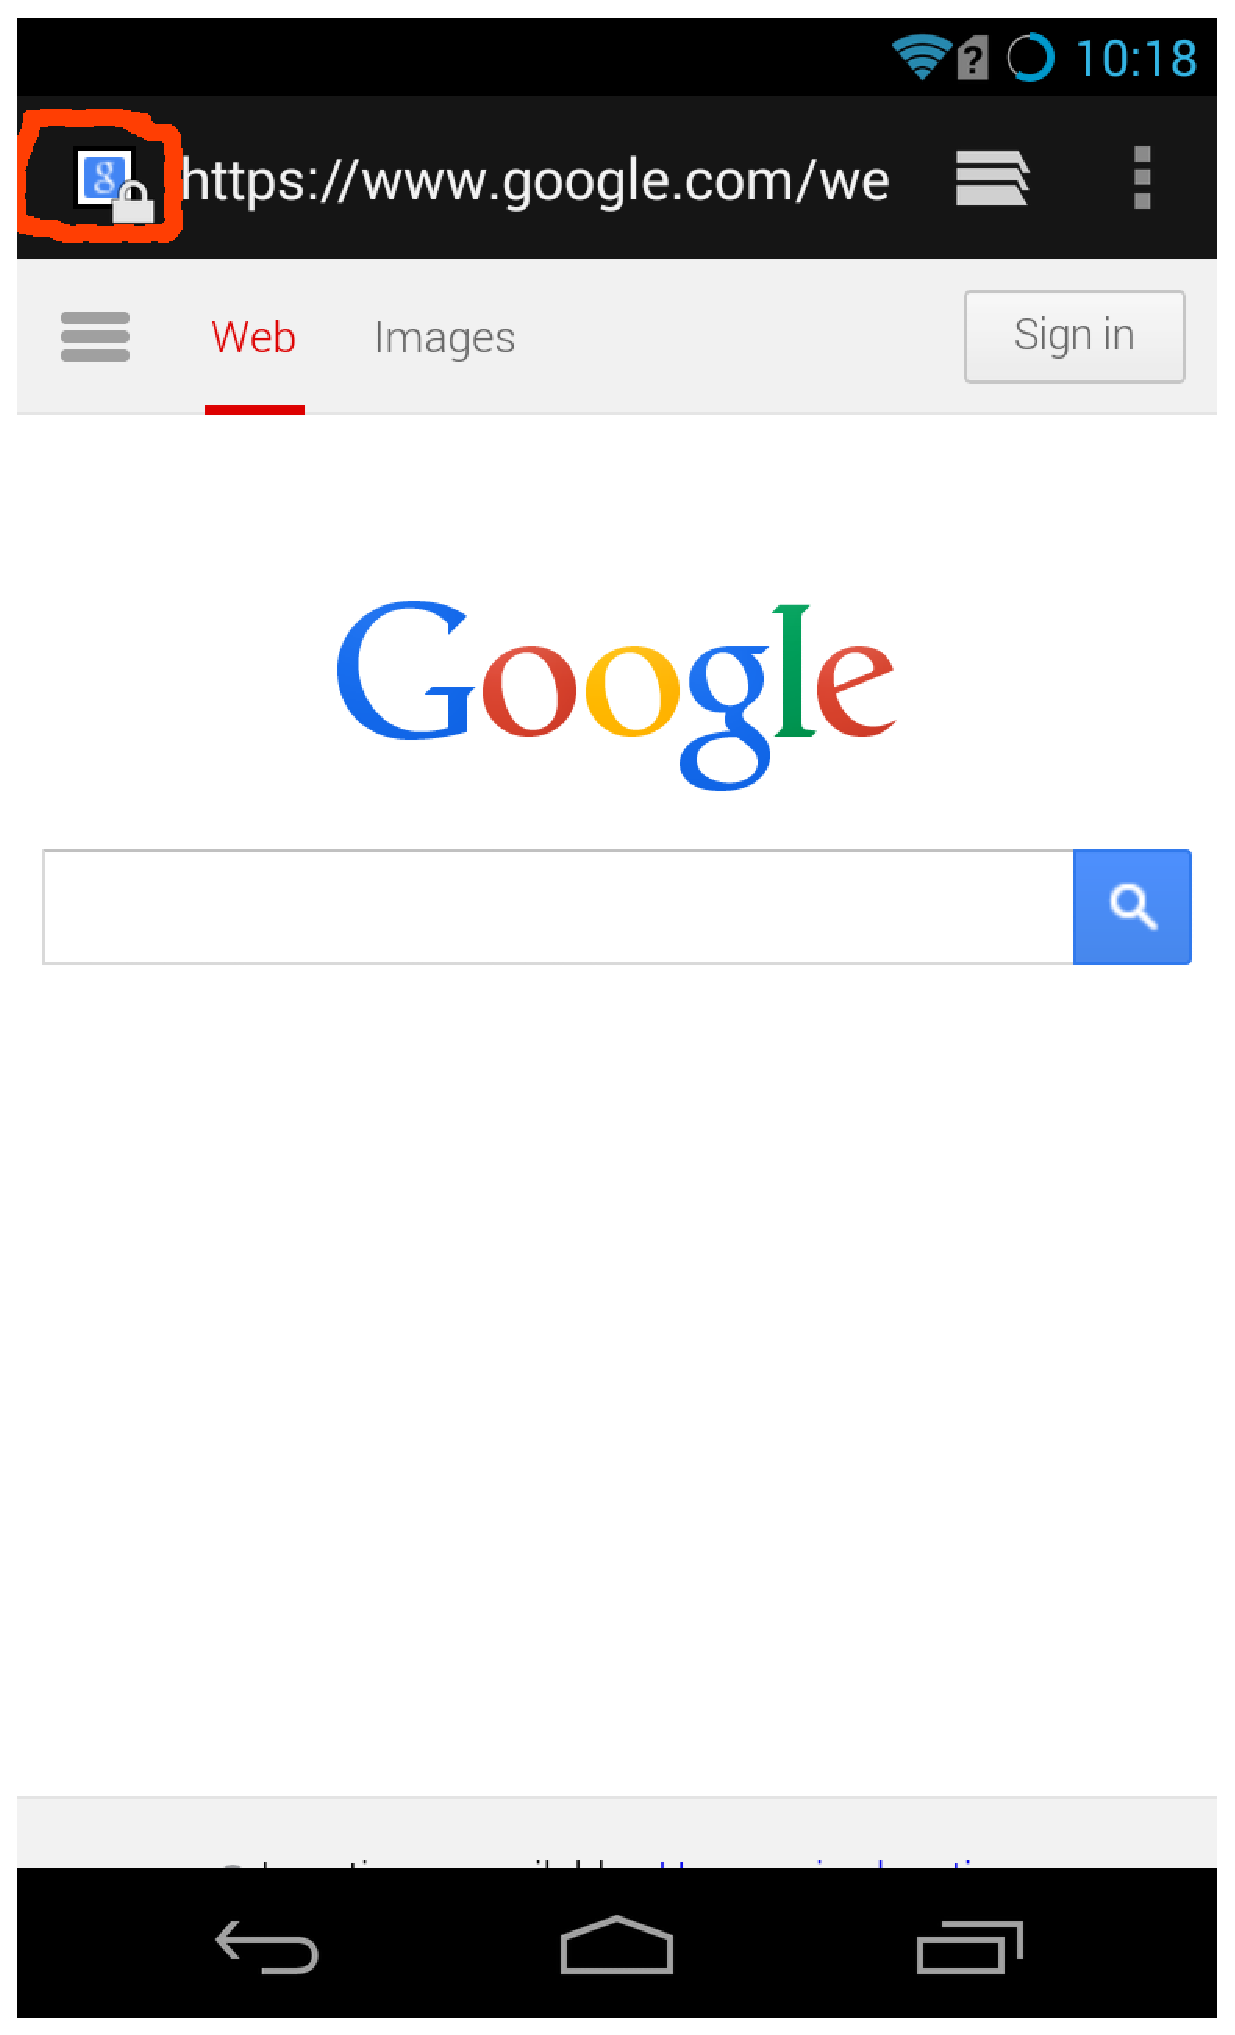
\includegraphics[scale=.24]{imgs/google-web-marked}\hspace{2em}
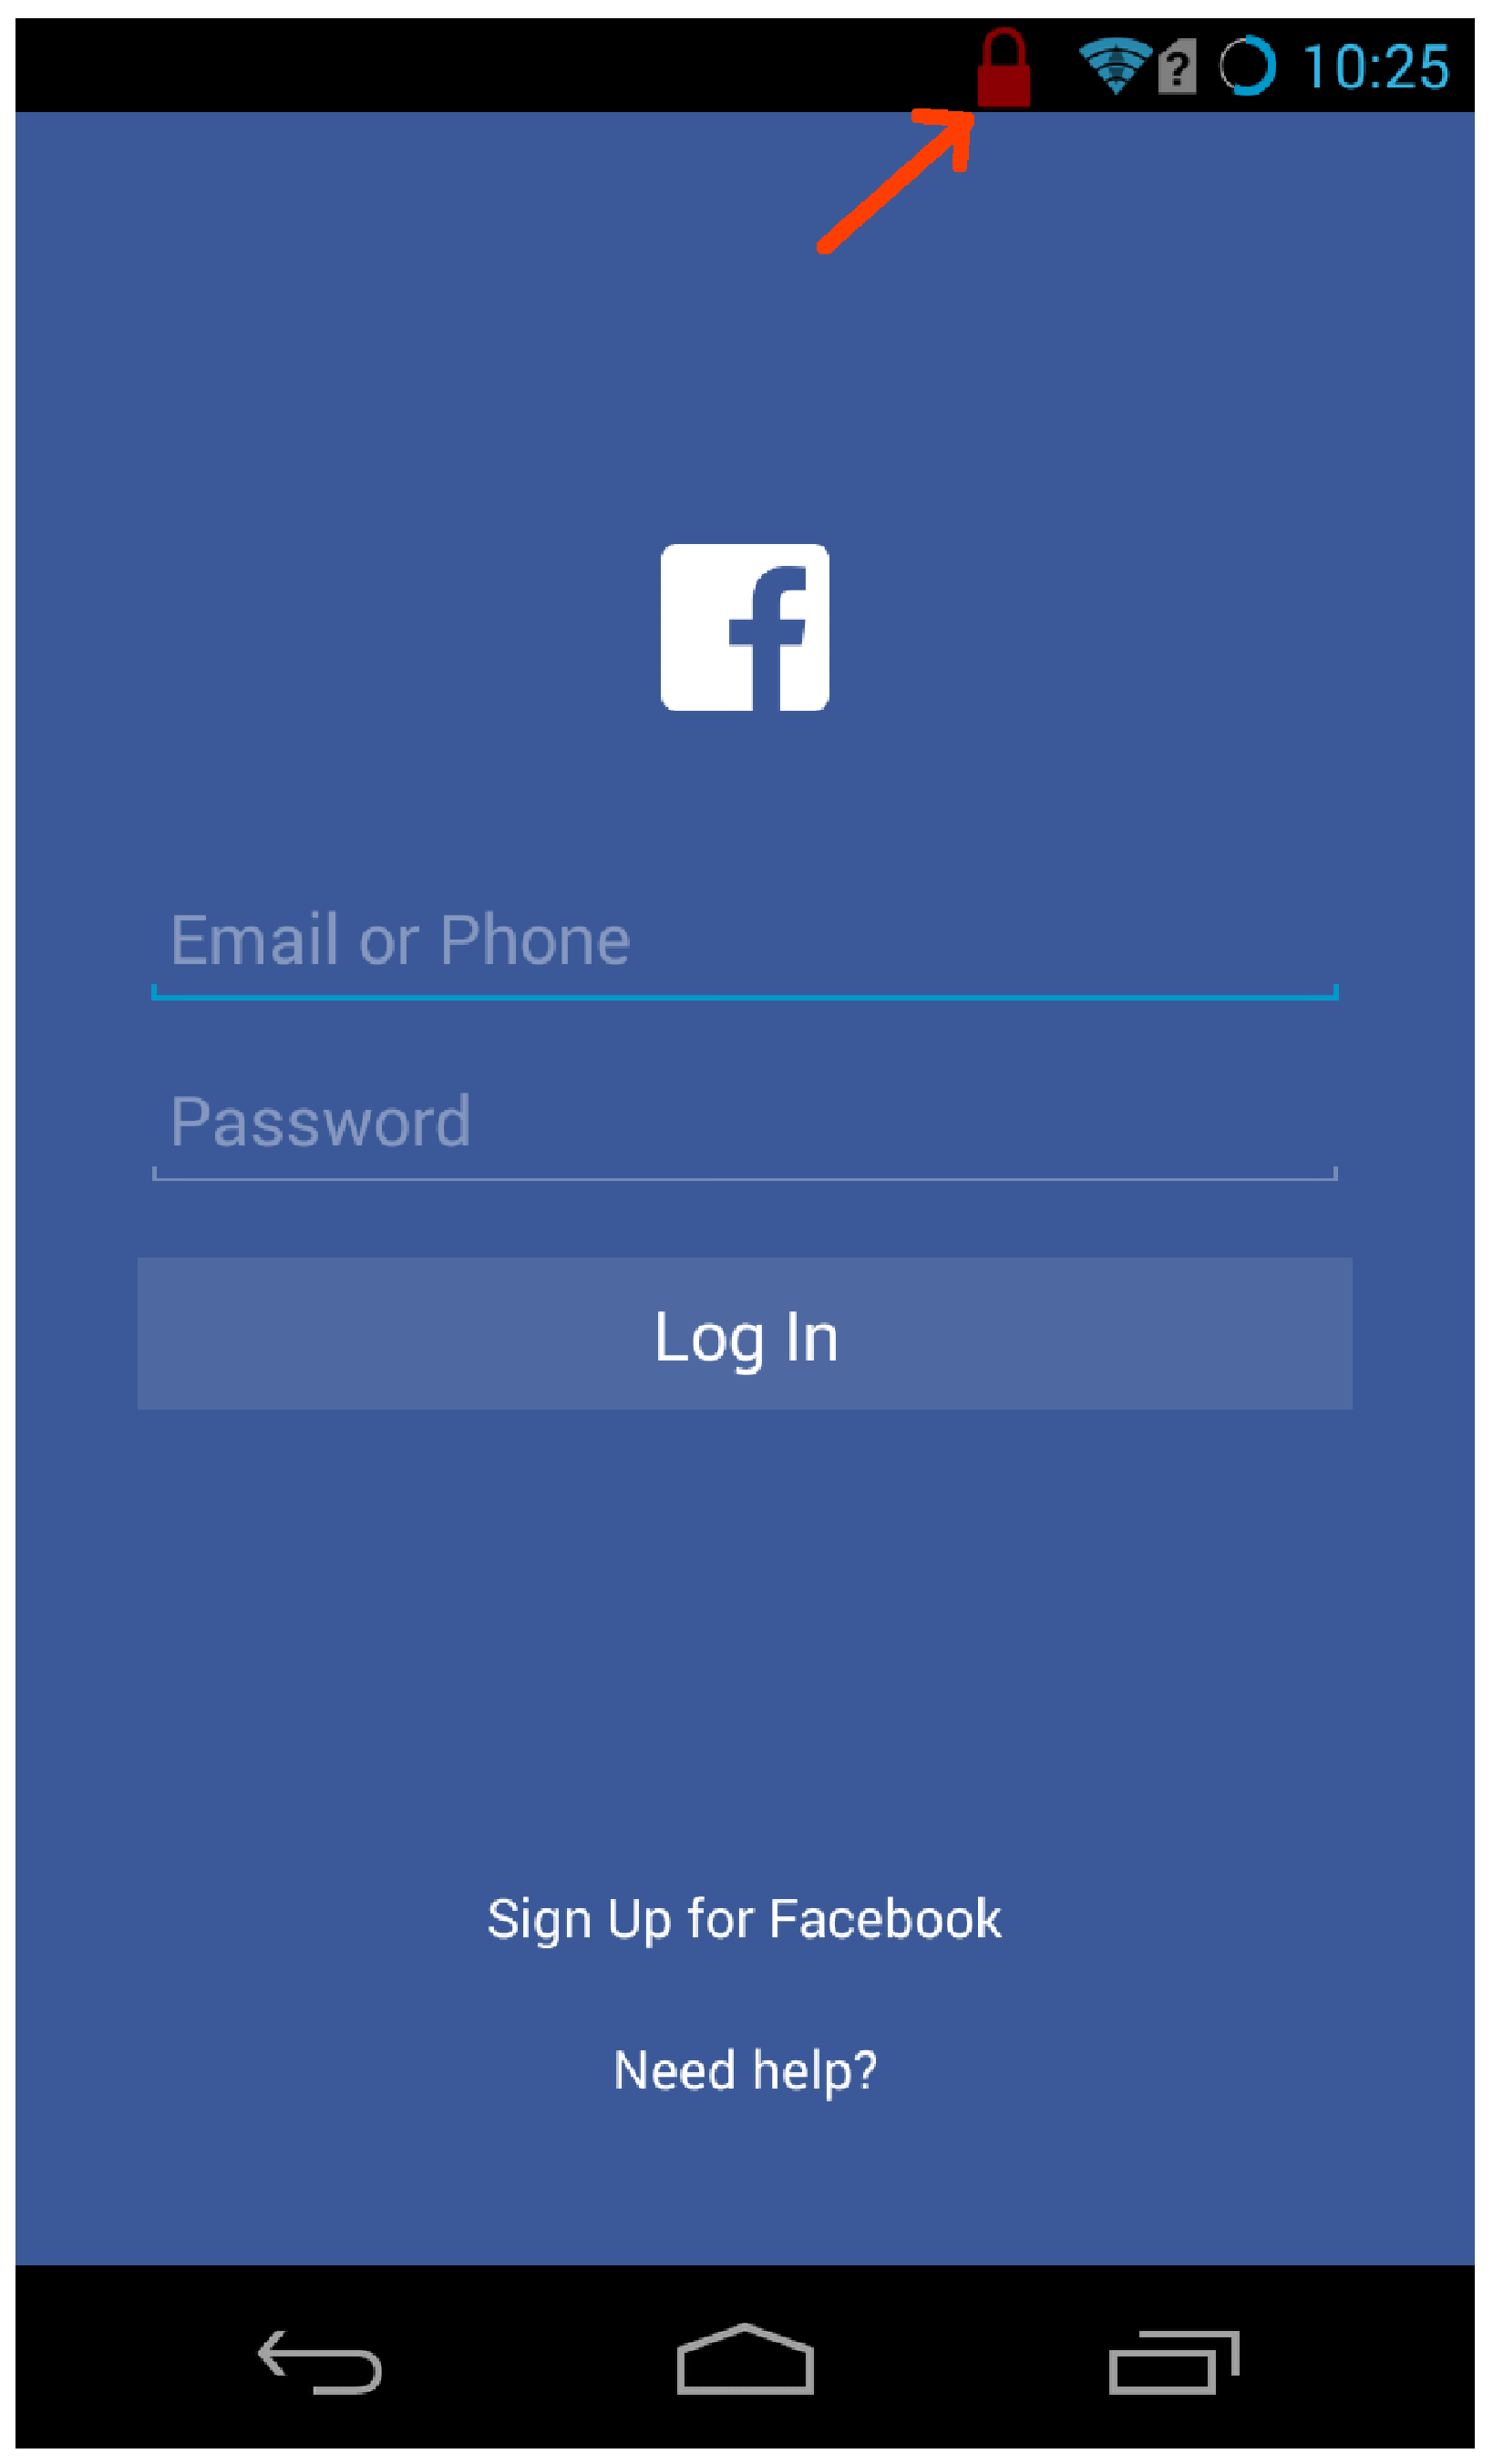
\includegraphics[scale=.18]{imgs/facebook-app-lock-1}
\\
\scriptsize (a) Padlock ahead URL (Web app)  \hskip 8em (b) Padlock on Android status bar (Proposed)
\caption{App padlock illustration}
\label{fig:padlock}
\end{figure}

In order to make the padlock symbol displayed whenever a secure connection is established, following steps of work should be done:
\begin{enumerate}
\item Collect all APIs of Android to make secure connection with the server
\item Monitor and intercept SSL/TLS related APIs of Android system
\item Tracking the handshake protocol of SSL/TLS protocol. Once they finish the handshake process, the padlock symbol should be displayed.
\end{enumerate}

%%-----------------------------------------------------------------------------
%% 	Reading materials
%%-----------------------------------------------------------------------------
\subsection{Reading materials}
A list of websites and papers related:
\begin{enumerate} 
\item Android framework source code. \cite{link_aosp}
\item Android secure connection frameworks. \cite{link_android_ssl}
\item To monitor and hook Android API calls, one possible method is by using Xposed \cite{link_xposed} framework.
\end{enumerate}
%%=============================================================================
%% 	Certificate Checker
%%=============================================================================
\section{SSL/TLS certificate checker}
\subsection{Android certificate checker description}

\begin{figure}[!htb]
\centering
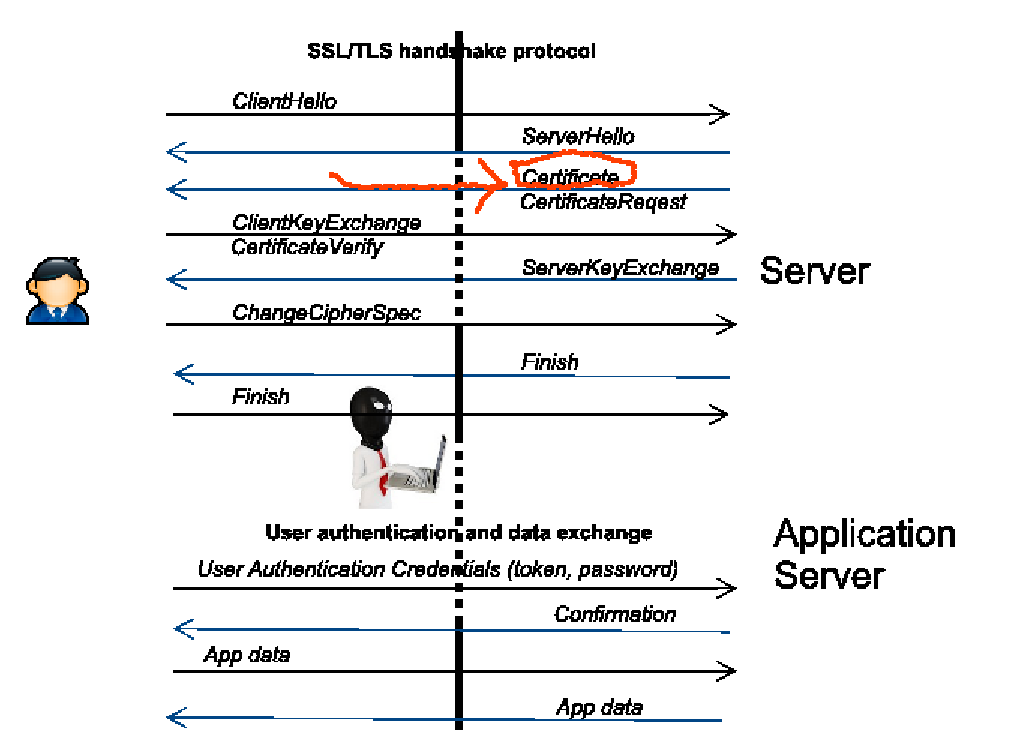
\includegraphics[scale=.5]{imgs/mitm_attack}
\caption{MITM attack process}
\label{fig:mitm}
\end{figure}
Figure \ref{fig:mitm} illustrates the MITM attack process. The attack only happens when the app doesn't check the 
certificate properly. According to \cite{fahl2012eve}, large amount of Android apps misuse the SSL/TLS and expose vulnerabilities to MITM attacks. These misuse of Android API includes:
\begin{itemize}
\item  Trusting all Certificates
\item Allowing all host names
\item Trusting too many CAs
\item Mixed-Mode/No SSL (SSL striping attack)
\end{itemize}
So we propose building the system level SSL/TLS certificate checker to enforce checking of the certificate by Android system.
For each app that is trying to establish SSL/TLS connection with the server, the checker will enforce certificate 
checking by examining the server certificate independently. The checker checks all but not limited to the following certificate use.
\begin{itemize}
\item Check certificate validation
\item Check CA that signs the certificate
\item Check target host name with the one in the certificate
\end{itemize}

%%-----------------------------------------------------------------------------
%% 	Reading materials
%%-----------------------------------------------------------------------------
\subsection{Reading materials}
A list of reading materials: 
\begin{itemize}
\item Why Eve and Mallory love Android: An analysis of Android SSL (in) security. \cite{fahl2012eve}
\item Paper on SSL/TLS Certificate \cite{akhawe2013here}.
\end{itemize}


%%------------------------------------------------------------------------------
%% References
%%------------------------------------------------------------------------------
\clearpage
\bibliographystyle {plain}
\bibliography{ssl}
\end{document}
